\begin{tikzpicture}[scale=1.5]
	%The spectra
	\node at (0,0) {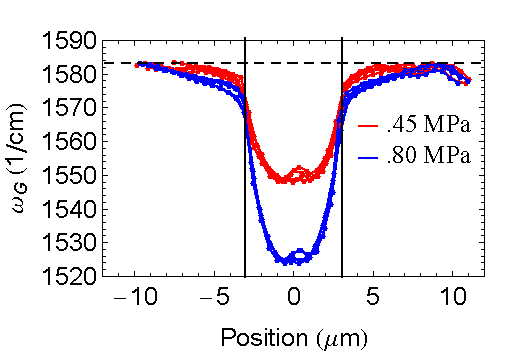
\includegraphics[scale=1.5]{Figs_Friction/QualLine.pdf}};
	
	%The picture of the hole
	\newcommand{\arrowlength}{1.5*.16*3.33 cm}
	\begin{scope}[xshift=-1.5 cm,yshift=0 cm]
		\node at (0,0) {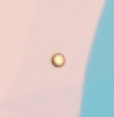
\includegraphics[scale=1.125,angle=0,trim=9.75mm 8.5mm 8.5mm 10.25mm,clip]{Figs_Friction/SB02-3_cropped.jpg}};
		\draw[black,thick] (0,\arrowlength) -- (0,-\arrowlength) ;
		\draw[black,thick] (\arrowlength,0) -- (-\arrowlength,0);
	\end{scope}
	
	%The picture of the SEM dot
	\begin{scope}[xshift=2.6 cm,yshift=-.8 cm]
		\node at (0,0) {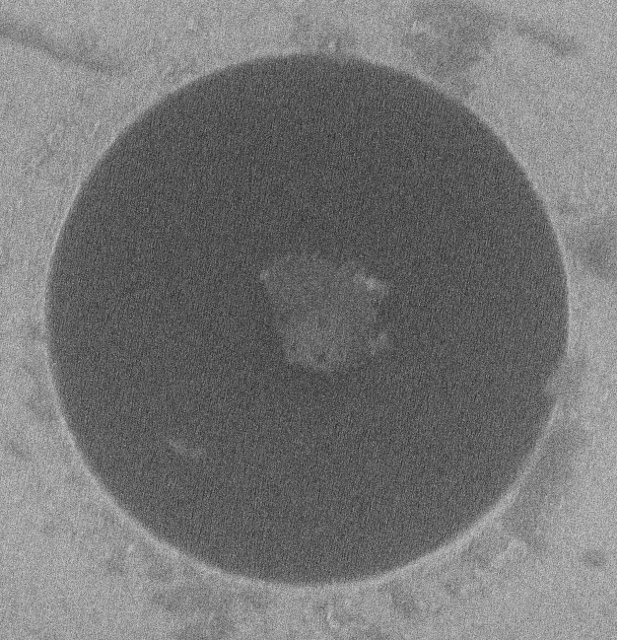
\includegraphics[width=.105 \textwidth]{Figs_Friction/SB02-3_05_SEM.jpg}};
	\end{scope}

\end{tikzpicture}